\begin{frame}
	\frametitle{Allgemein}
	
\textbf{Aufgabenstellung:}

Entwickeln eines Mini-Java Compilers mit den zugehörigen Schritten: Lexer, Parser, TypChecker und Codegenerierung.
\end{frame}

\begin{frame}[fragile]
\frametitle{Allgemein: Ziel}

\textbf{Ziel} 

Korrektes Übersetzen der folgenden Klasse:

\begin{lstlisting}[language=Java]
class Fibonacci {
  int getFib(int n) {
    return (n < 2) ? n : getFib(n-1) + getFib(n-2);
  }
}
\end{lstlisting}	
\end{frame}



\begin{frame}{Featureliste}

Umgesetze Features (Auszug):

\begin{itemize}
	\item Ternary Operator
	\item For / While / DoWhile 
	\item If / If-Else / Switch-Case
	\item Pre- bzw. Post Inkrement/Dekrement
	\item Arithmetische Operatoren (+, -, /, div, mod, *) inklusive Zuweisung (+=, etc.)
\end{itemize}	
\end{frame}

\begin{frame}{Entwicklung}

Code-Sharing über GitHub (https://github.com/Pfeifenjoy/compilerbau-WS17-18) mit continuous integration (travis).

\par \medskip

Als Build-System wird cabal eingesetzt.	
\end{frame}

\begin{frame}{Projektmanagement}

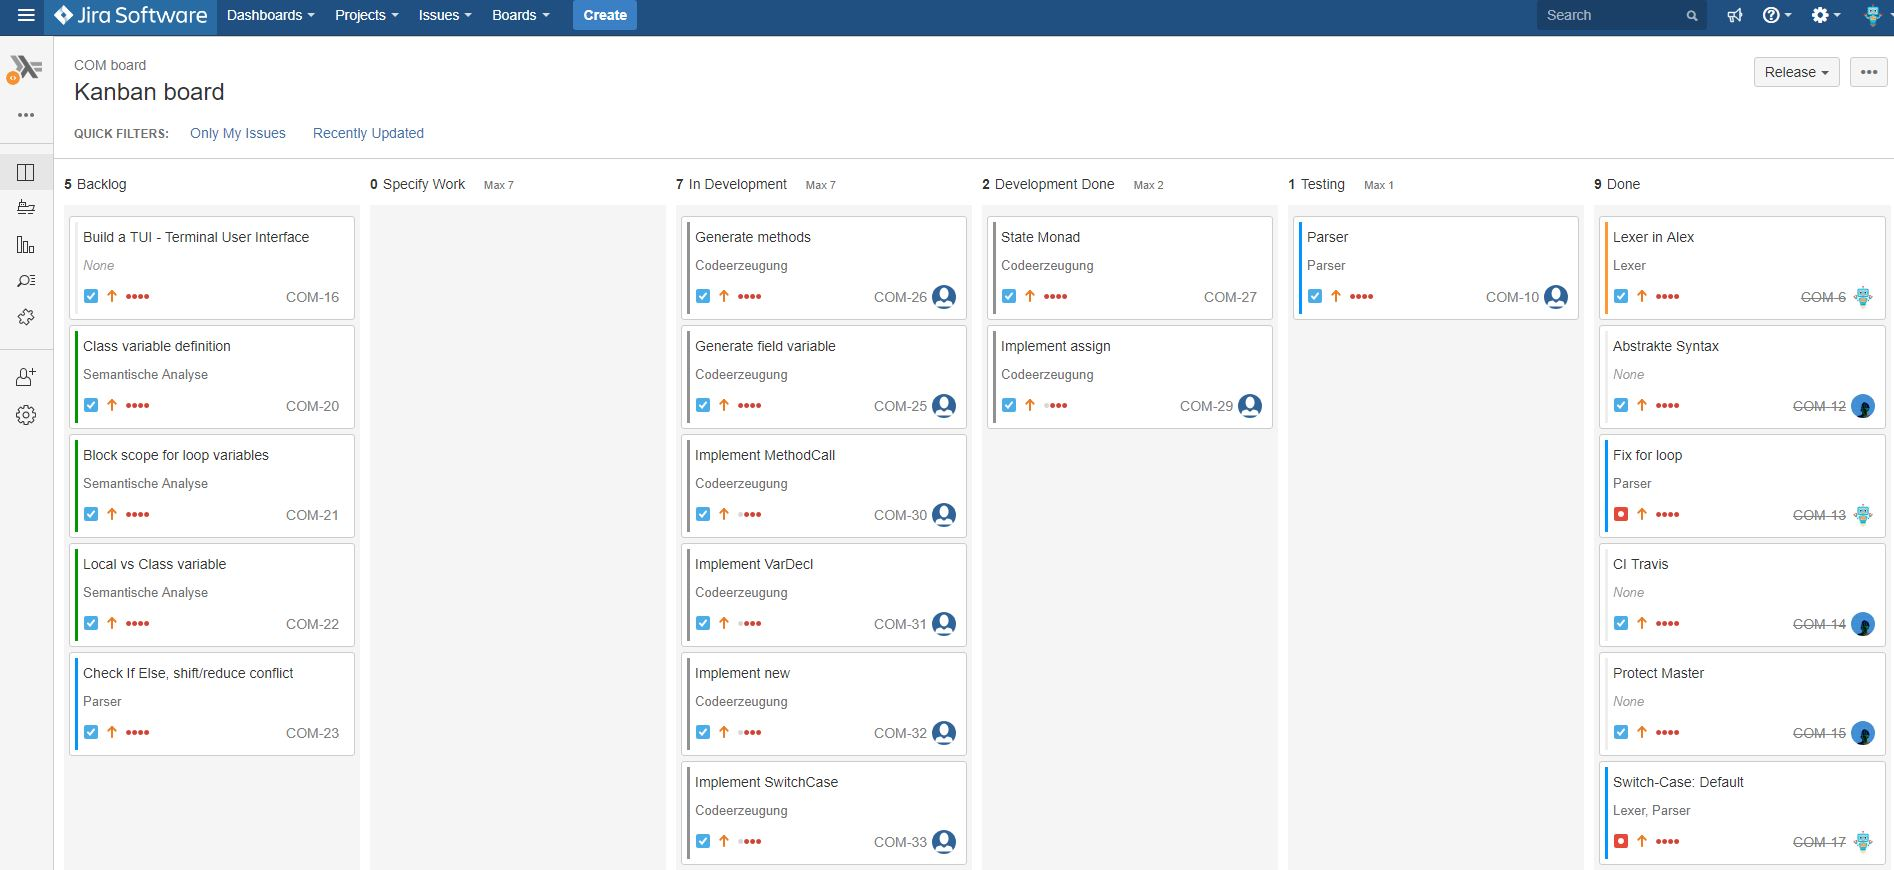
\includegraphics[scale=0.25]{images/jira.jpg}

\end{frame}
